\newpage
\section{Scenario 3 - Above the GS}\label{sec:scenario3}
The scenario 3 run in a short distance from north to south, where the Unmanned Aircraft flies over the Ground Station. The UA starts and ends 6km from the GS from North to South as can be seen in Figure \ref{fig:s3_losa}. The distance between the 2 devices at every sample is shown in Figure \ref{fig:s3_losc}. As follows in former graphs, the blue circles mean that there is line of sight between them. 


\begin{figure}[H]
	\centering
	\subfigure[UAS Map Positioning]{\label{fig:s3_losa} 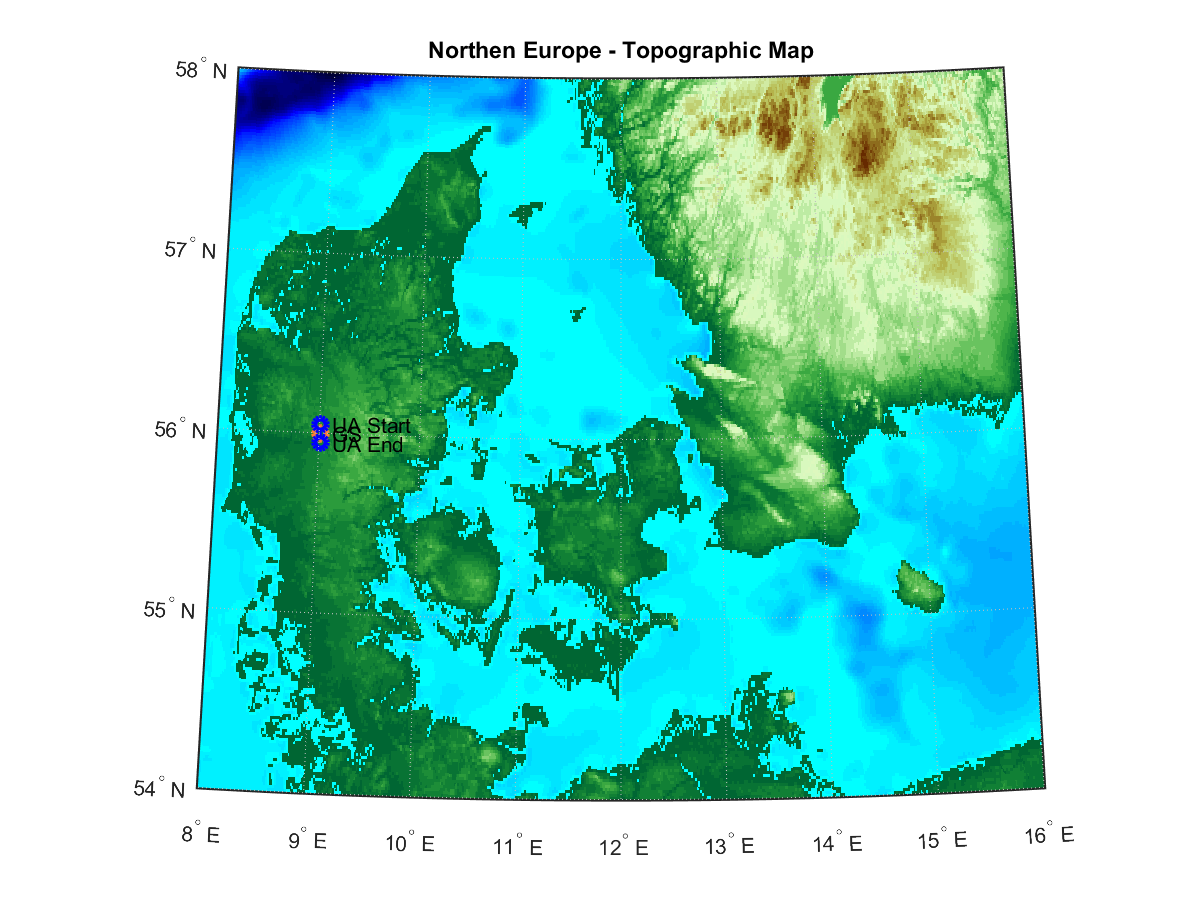
\includegraphics[scale=0.36]{figures/s3_map.png}}
	\subfigure[UAS Map Zoom]{\label{fig:s3_losb} 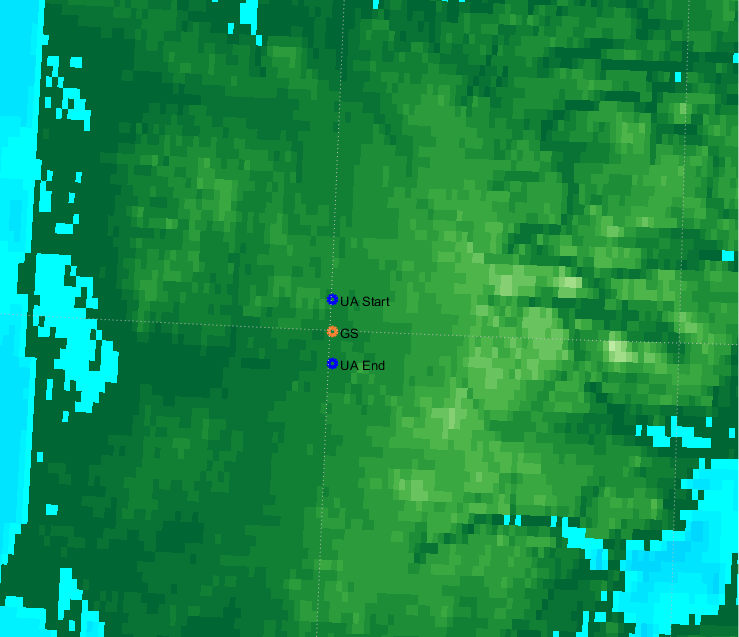
\includegraphics[scale=0.32]{figures/s3_zoom.png}}
	\\
	\subfigure[LOS and Distance]{\label{fig:s3_losc} 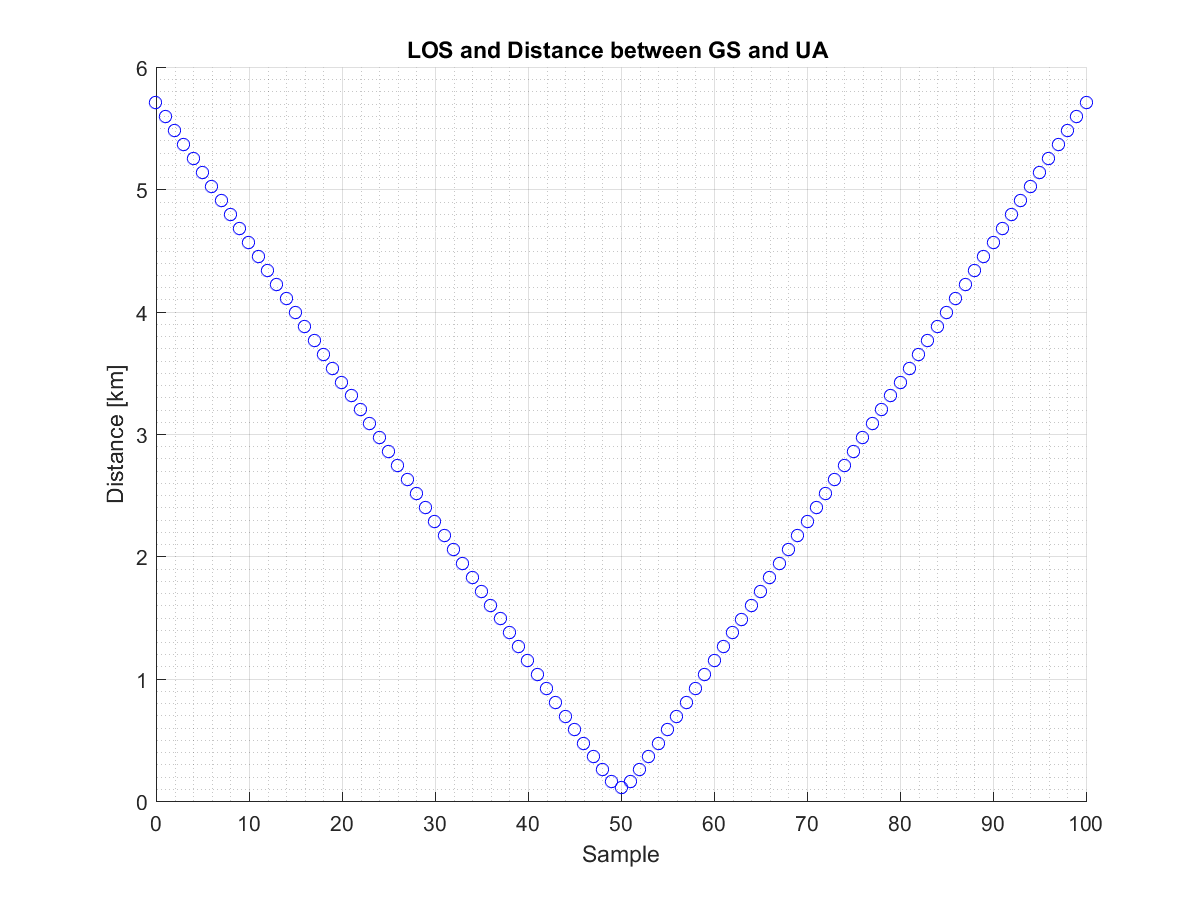
\includegraphics[scale=0.53]{figures/s3_los.png}}
	\caption{Above the GS Scenario}
	\label{fig:s3_map}
\end{figure}

\subsection*{UA and GS Tracking Angles}
In the start of the simulation, both Ground Station and Unmanned Aircraft calculate their azimuth and elevation angles necessary to point at each other (optimal angles). A small delay can be seen on Figure \ref{fig:s3_gs} for $\theta_{GS}$ to reach $\theta_{OPTIMAL}$. This delay is the result of the starting point of the antennas, being 0$^{\circ}$, and the motion of the moving angle system. Hence, no delay can be observed for the azimuth angle of the UA and the elevation angles of both devices, by cause of having 0$^{\circ}$ for their optimal angle and their starting angle (Figures \ref{fig:s3_ua} and \ref{fig:s3_gs}).

The crossing point can be clearly observed on their elevation angles, where the speed of the aircraft is directly related to their sudden changes, resulting in a quick peak of almost -90 and 90 degrees for respectively, the UA and the GS. 

\begin{figure}[H]
	\centering
	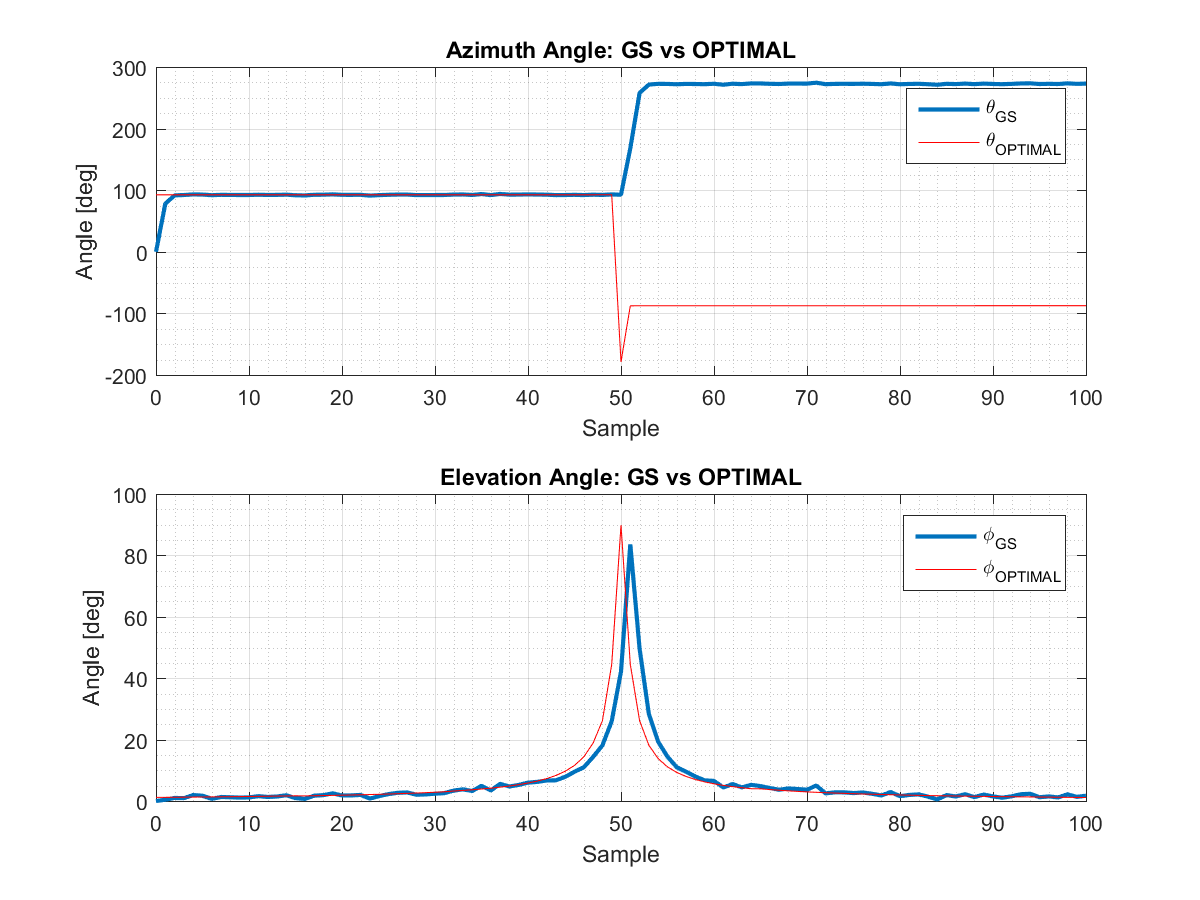
\includegraphics[scale=0.8]{figures/s3_gs.png}
	\caption{Azimuth and elevation angles of GS following the optimal angle}
	\label{fig:s3_gs}
\end{figure}

\begin{figure}[H]
	\centering
	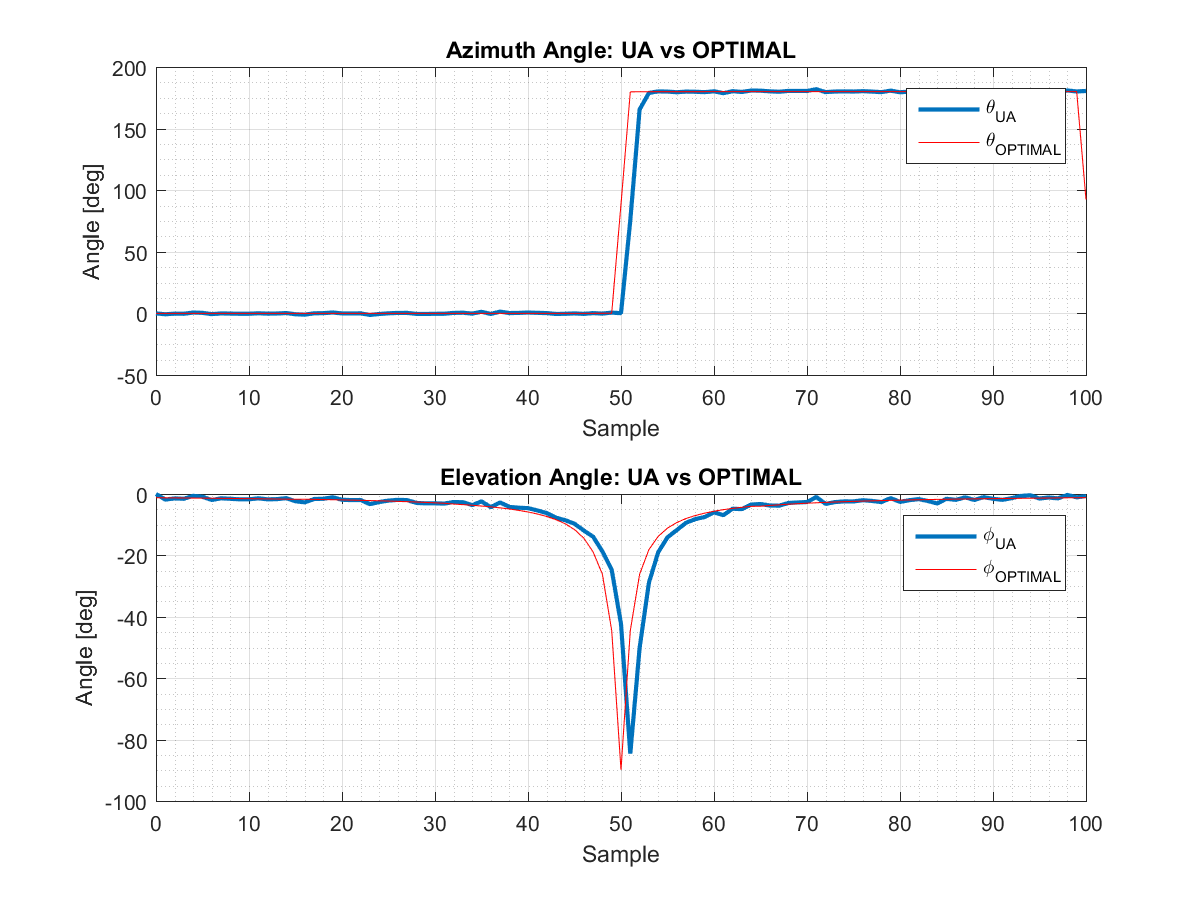
\includegraphics[scale=0.8]{figures/s3_ua.png}
	\caption{Azimuth and elevation angles of UA following the optimal angle}
	\label{fig:s3_ua}
\end{figure}

\subsection*{Signal Power}
In Figure \ref{fig:s3_power}, the power at the receiver is growing in time. While the UA is moving in the direction of the GS, the distance between them decreases and thus the power in the receiver increases. However, a drop-off can be seen at their crossing point (Time sample 52). At this point, both moving angle system are not fast enough to react on the high speed of the UA. Thus, at their crossing point, the antennas of the two devices will not point directly at each other, having for effect to decrease the power in the receiver.

\begin{figure}[H]
	\centering
	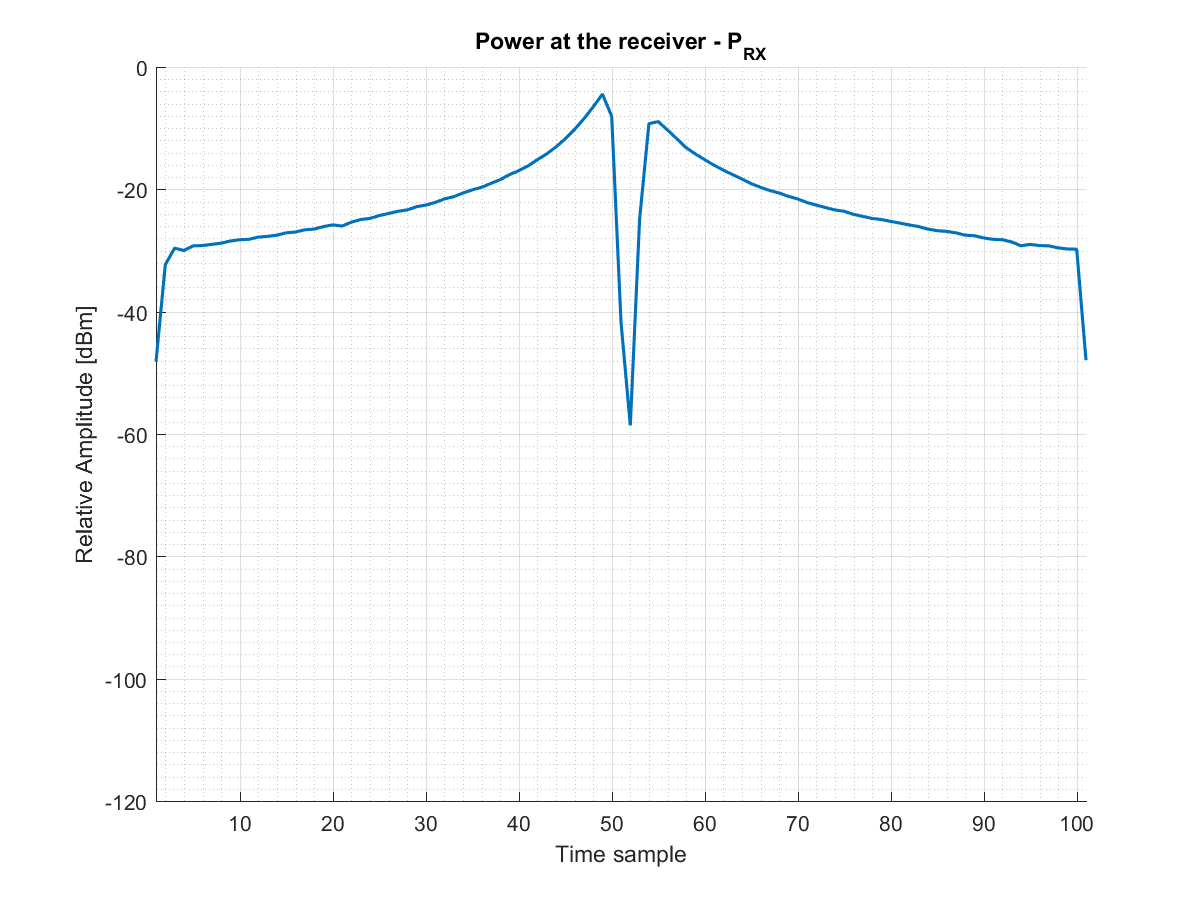
\includegraphics[scale=0.8]{figures/s3_power.png}
	\caption{Power at the receiver's antenna at both ends}
	\label{fig:s3_power}
\end{figure}